\documentclass{article}
\usepackage{gensymb, amsmath, float, graphicx, epstopdf}
\restylefloat{table}
\usepackage[margin=0.75in]{geometry}
\begin{document}

\title{Lab Write-up 4: Shielded-Loop Resonators}
\author{Michael Shen}
\maketitle


\section{Finding the Resonant Frequency}

\subsection{Measured Data}

\begin{table}[H]
\centering
\begin{tabular}{|c|c|c|}
\hline
Loop & $f_0$ (MHz) & $\vert\Gamma^{\prime}_{in}\vert$ \\ \hline
5 cm & 89.209 & 0.237 \\ \hline
9 cm & 49.774 & 0.260 \\ \hline
\end{tabular}
\end{table}

\subsection{Questions}

\begin{enumerate}
	\item Since $C \approx C^{\prime}l$, the longer, 9 cm, loop should have a greater capacitance.
	\item Since $L = \mu r [ln \frac{32r}{d}-1.75]$ for shielded-loop resonators and $\mu$ and $d$ are constant between the loops, the loop with the larger radius, the 9 cm loop, should have a greater inductance.
	\item Since $f_0 = \dfrac{\omega_0}{2\pi}$ and $\omega_0 = \dfrac{1}{\sqrt{LC}}$, the loop with the smaller $LC$ product will have a higher resonant frequency. Since the 5cm loop should have both a smaller $C$ and $L$, it should have a higher resonant frequency. This is confirmed by our experimental results as the 5 cm loop has a resonant frequency of 89.209 MHz compared to a resonant frequency of 49.774 MHz for the 9 cm loop.
\end{enumerate}


\section{De-embedding the Feedline}

\subsection{Measured Data}
\begin{table}[H]
\centering
\begin{tabular}{|c|c|c|c|}
\hline
Loop & $\vert\Gamma^{\prime}_{in}\vert$ & $\vert\Gamma^{\prime}_{in}\vert$ at $f_0$ - 2MHz & $\vert\Gamma^{\prime}_{in}\vert$ at $f_0$ + 2MHz \\ \hline
5 cm & 0.9735\angle 109.9\degree & 0.9745\angle 123.5\degree & 0.9744\angle 96.61\degree \\ \hline
9 cm & 0.9712\angle 118.1\degree & 0.9745\angle 143.6\degree & 0.9772\angle 93.61\degree \\ \hline
\end{tabular}
\end{table}

\subsection{Analysis}
\begin{enumerate}
	\item $\beta l_{5cm}$: $180 - 2\beta l = 109.9\degree \Rightarrow \beta l = 35.95\degree = 0.63 rad$ \\
		  $\beta l_{9cm}$: $180 - 2\beta l = 118.1\degree \Rightarrow \beta l = 31.45\degree = 0.55 rad$ \\
	\item $\beta l_{5cm}$ at $f_0 - 2 MHz = \beta l\times\dfrac{f_0 - 2MHz}{f_0} = 0.62 rad$ \\
		  $\beta l_{5cm}$ at $f_0 + 2 MHz = \beta l\times\dfrac{f_0 + 2Mhz}{f_0} = 0.64 rad$ \\
		  $\beta l_{9cm}$ at $f_0 - 2 MHz = \beta l\times\dfrac{f_0 - 2MHz}{f_0} = 0.53 rad$ \\
		  $\beta l_{9cm}$ at $f_0 + 2 MHz = \beta l\times\dfrac{f_0 + 2Mhz}{f_0} = 0.57 rad$ \\ 
	\item $\beta_{5cm} = \dfrac{\omega_0\sqrt{\varepsilon_r}}{c} = \dfrac{2\pi\times89.209\times10^6\times\sqrt{2.2}}{3.0\times10^8} = 2.77$ \\
	$\beta_{9cm} = \dfrac{\omega_0\sqrt{\varepsilon_r}}{c} = \dfrac{2\pi\times49.774\times10^6\times\sqrt{2.2}}{3.0\times10^8} = 1.55$
	\item $l_{5cm} = 4 + \pi r = 4 + 5\pi = 19.7 cm$ \\
	      $l_{9cm} = 5 + \pi r = 5 + 9\pi = 33.3 cm$ \\
	\item $\beta l_{5cm} = 2.77\times19.7 = 54.6 rad$ \\
		  $\beta l_{9cm} = 1.55\times33.3 = 51.6 rad$ \\
\end{enumerate}

\subsection{Questions}
\begin{enumerate}
	\item The 5 cm loop has a feedline with larger electrical length. $\beta = \omega\sqrt{L'C'}$. Since $\omega_0 = \dfrac{1}{\sqrt{LC}}$ and $L'C' = \dfrac{LC}{l^2}$, $\beta = \dfrac{1}{l}$ and $\beta l = 1$. Therefore, electrical length is independent of feedline length, so it is possible that the 5 cm loop does indeed have a larger electrical length.
	\item Both reflection coefficients are high, but the 9 cm loop had the higher reflection coefficient. We should desire a large magnitude of input reflection coefficient so that the line can be matched. For a lossless resonator, $\vert S_{11} \vert = 1$.
\end{enumerate}


\section{Finding R, L, and C}

\subsection{Measured Data}
\begin{table}[H]
\centering
\begin{tabular}{|l|l|l|l|}
\hline
Loop & R & L & C \\ \hline
5 cm & 0.671 $\Omega$  & 0.194 H  & $2.77\times10^{-5}$ F \\ \hline
9 cm & 0.731 $\Omega$  & 0.457 H & $3.08\times10^{-5}$ F \\ \hline
\end{tabular}
\end{table}

\subsection{Analysis}
$X_{a5} = 40.63$ \\
$X_{a9} = 28.91$ \\
$X_{b5} = 48.40$ \\
$X_{b9} = 48.76$ \\
$Q_{5cm} = 124.72$ \\
$Q_{9cm} = 166.41$ \\
\begin{enumerate}
	\item $L_{5cm} = \mu r[ln\dfrac{32r}{d} - 1.75] = 1.83\times 10^-7 H$ \\
		  $L_{9cm} = \mu r[ln\dfrac{32r}{d} - 1.75] = 3.9\times 10^-7 F$
	\item
\end{enumerate}

\subsection{Questions}

\begin{enumerate}
	\item 
	\item 
	\item 
\end{enumerate}

%\section{Figures and Images}
%\begin{figure}[H]
%    \centering
%    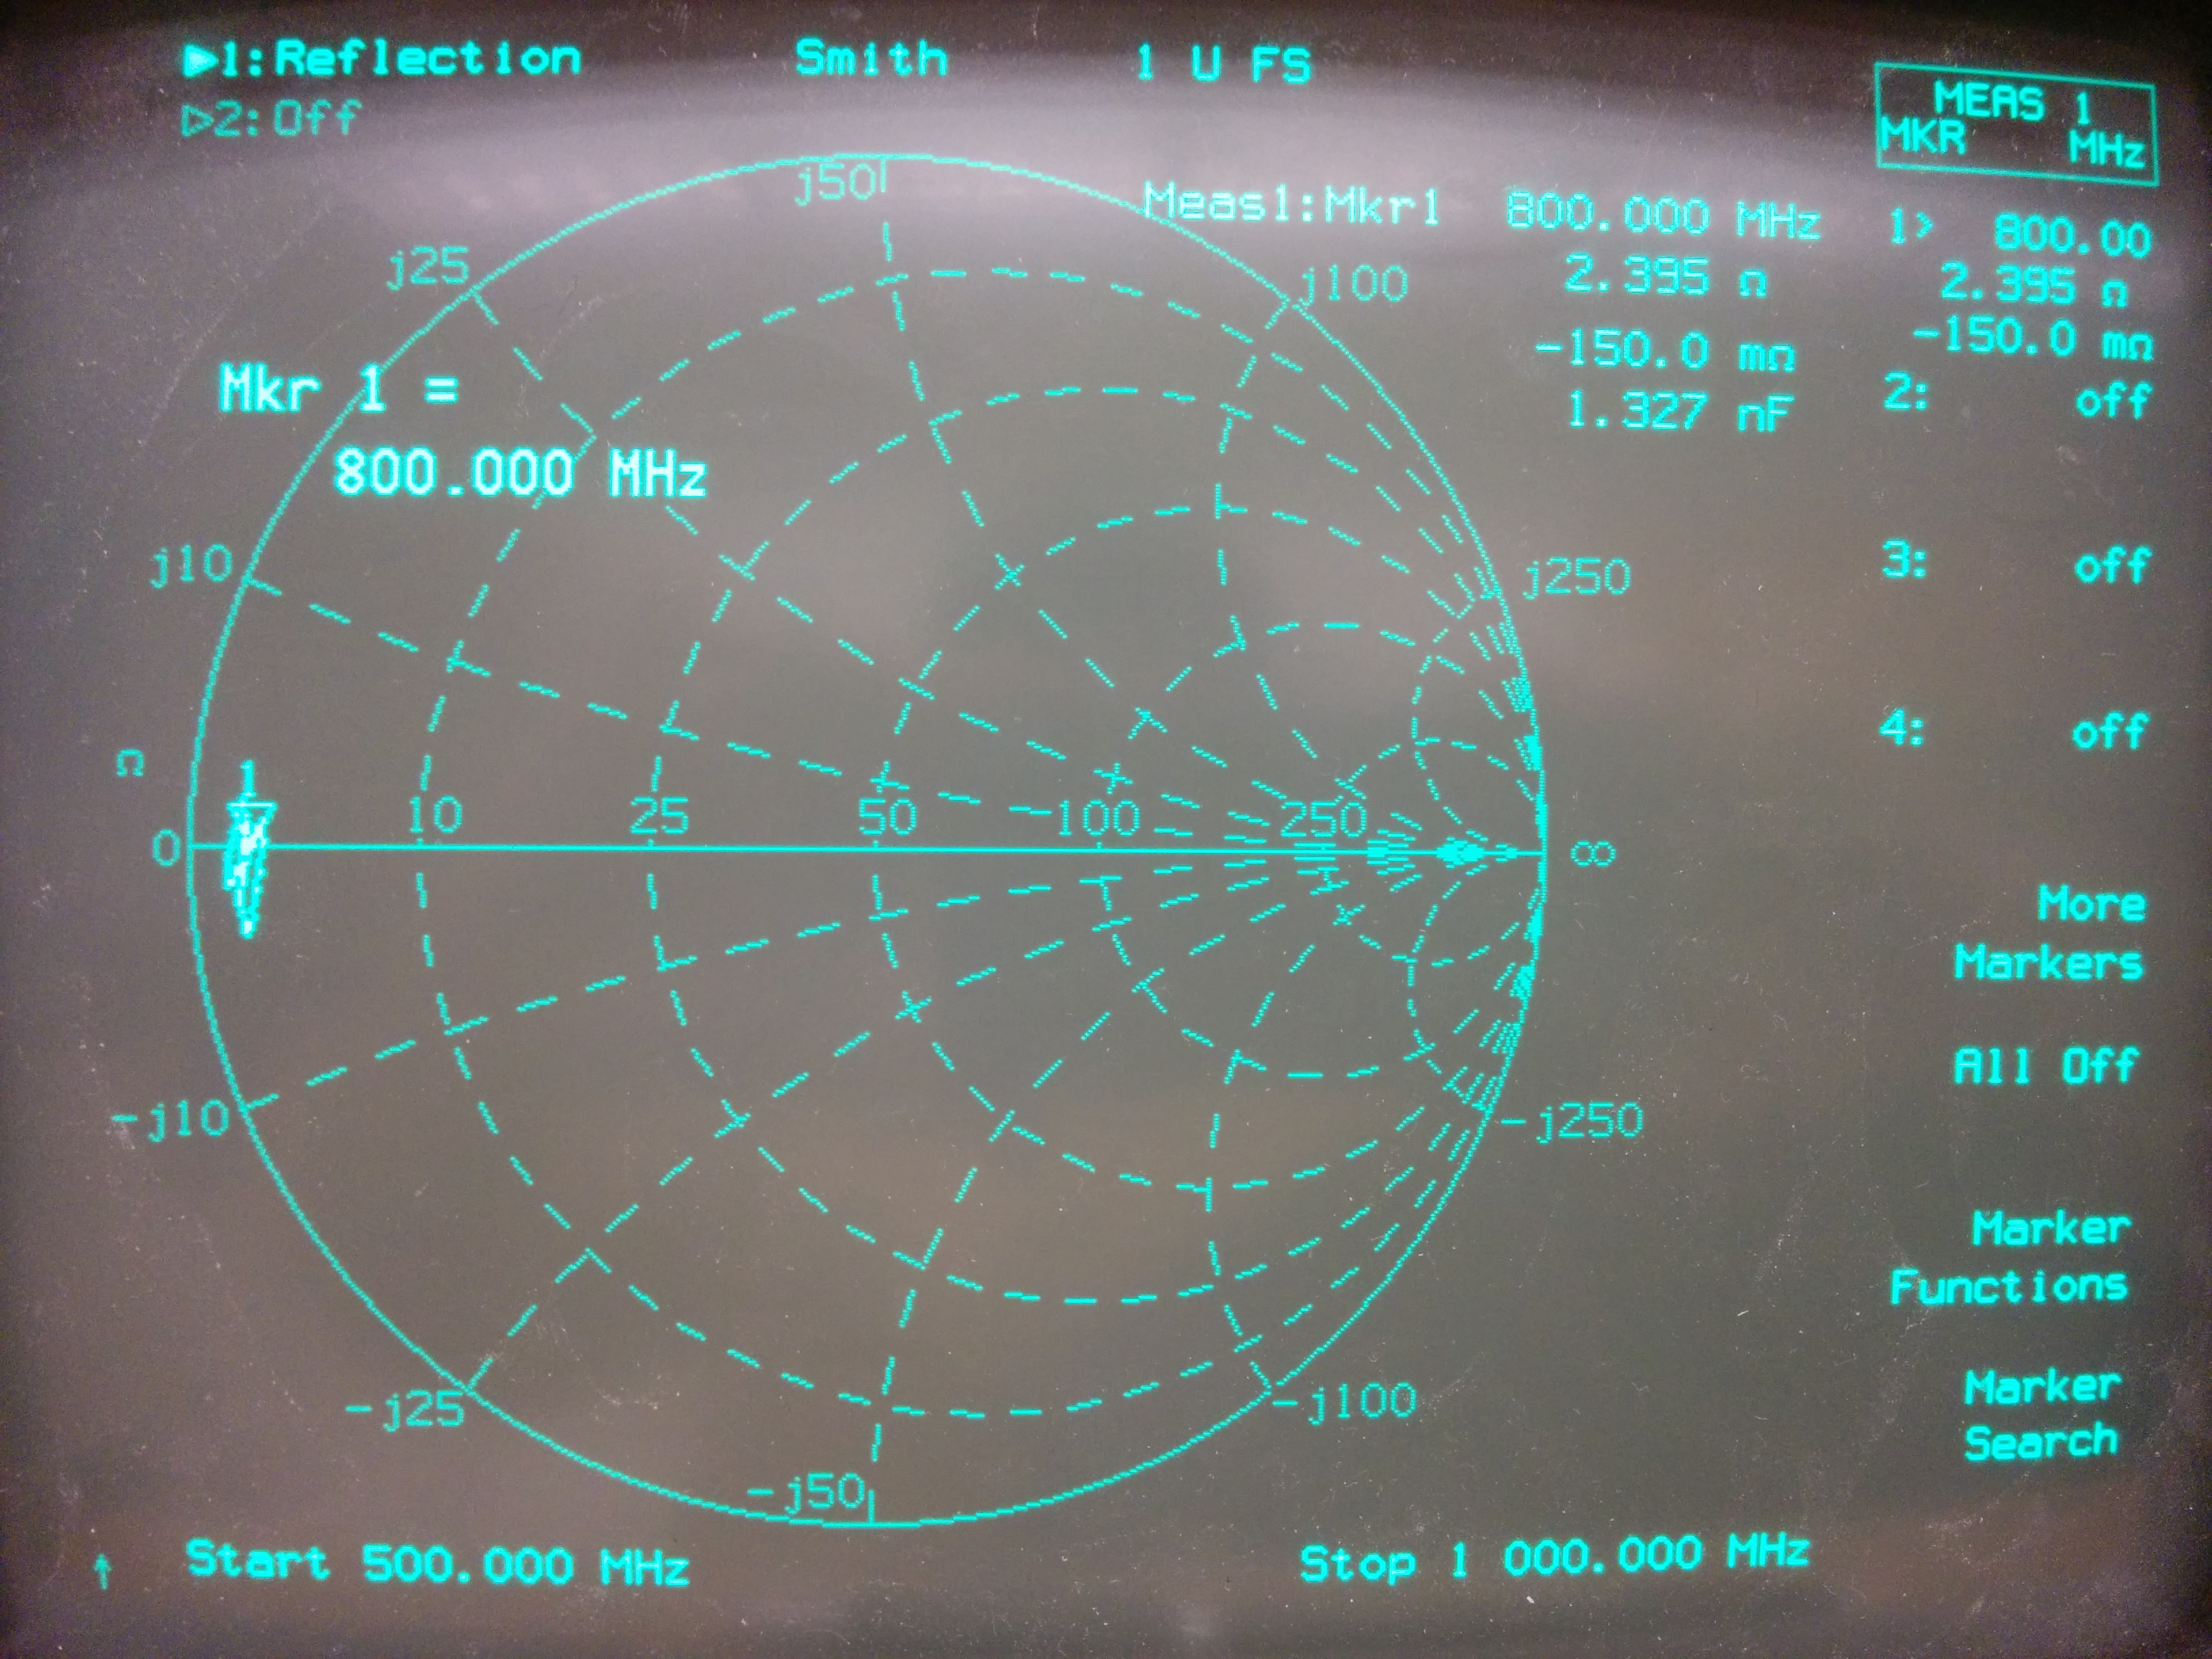
\includegraphics[width=0.8\textwidth]{./Images/251.jpg}
%    \caption{Point-like response for a lossless line}
%\end{figure}

\end{document}